\documentclass[tikz,border=4pt]{standalone}
\begin{document}
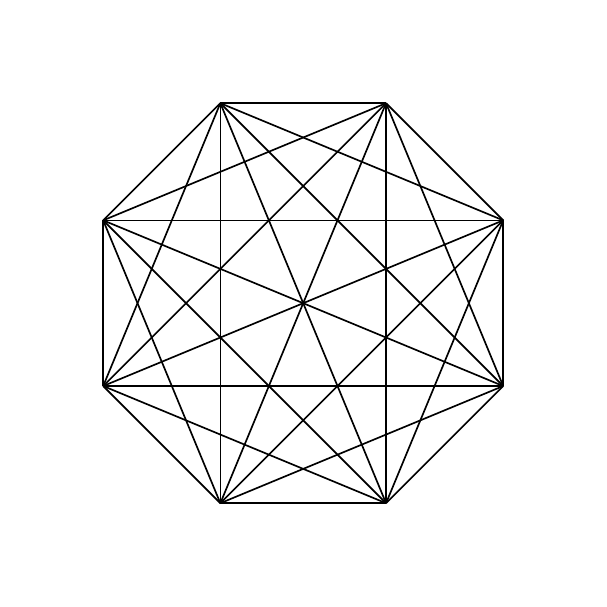
\begin{tikzpicture}[x=0.025cm,y=-0.025cm]
\path[use as bounding box] (0,0) rectangle (280,280);
\path[draw=black,fill=none,line width=0.6pt,line join=round] (241.6267,182.0952) -- (182.0952,241.6267);
\path[draw=black,fill=none,line width=0.6pt,line join=round] (241.6267,182.0952) -- (97.9048,241.6267);
\path[draw=black,fill=none,line width=0.6pt,line join=round] (241.6267,182.0952) -- (38.3733,182.0952);
\path[draw=black,fill=none,line width=0.6pt,line join=round] (241.6267,182.0952) -- (38.3733,97.9048);
\path[draw=black,fill=none,line width=0.6pt,line join=round] (241.6267,182.0952) -- (97.9048,38.3733);
\path[draw=black,fill=none,line width=0.6pt,line join=round] (241.6267,182.0952) -- (182.0952,38.3733);
\path[draw=black,fill=none,line width=0.6pt,line join=round] (241.6267,182.0952) -- (241.6267,97.9048);
\path[draw=black,fill=none,line width=0.6pt,line join=round] (182.0952,241.6267) -- (97.9048,241.6267);
\path[draw=black,fill=none,line width=0.6pt,line join=round] (182.0952,241.6267) -- (38.3733,182.0952);
\path[draw=black,fill=none,line width=0.6pt,line join=round] (182.0952,241.6267) -- (38.3733,97.9048);
\path[draw=black,fill=none,line width=0.6pt,line join=round] (182.0952,241.6267) -- (97.9048,38.3733);
\path[draw=black,fill=none,line width=0.6pt,line join=round] (182.0952,241.6267) -- (182.0952,38.3733);
\path[draw=black,fill=none,line width=0.6pt,line join=round] (182.0952,241.6267) -- (241.6267,97.9048);
\path[draw=black,fill=none,line width=0.6pt,line join=round] (97.9048,241.6267) -- (38.3733,182.0952);
\path[draw=black,fill=none,line width=0.6pt,line join=round] (97.9048,241.6267) -- (38.3733,97.9048);
\path[draw=black,fill=none,line width=0.6pt,line join=round] (97.9048,241.6267) -- (97.9048,38.3733);
\path[draw=black,fill=none,line width=0.6pt,line join=round] (97.9048,241.6267) -- (182.0952,38.3733);
\path[draw=black,fill=none,line width=0.6pt,line join=round] (97.9048,241.6267) -- (241.6267,97.9048);
\path[draw=black,fill=none,line width=0.6pt,line join=round] (38.3733,182.0952) -- (38.3733,97.9048);
\path[draw=black,fill=none,line width=0.6pt,line join=round] (38.3733,182.0952) -- (97.9048,38.3733);
\path[draw=black,fill=none,line width=0.6pt,line join=round] (38.3733,182.0952) -- (182.0952,38.3733);
\path[draw=black,fill=none,line width=0.6pt,line join=round] (38.3733,182.0952) -- (241.6267,97.9048);
\path[draw=black,fill=none,line width=0.6pt,line join=round] (38.3733,97.9048) -- (97.9048,38.3733);
\path[draw=black,fill=none,line width=0.6pt,line join=round] (38.3733,97.9048) -- (182.0952,38.3733);
\path[draw=black,fill=none,line width=0.6pt,line join=round] (38.3733,97.9048) -- (241.6267,97.9048);
\path[draw=black,fill=none,line width=0.6pt,line join=round] (97.9048,38.3733) -- (182.0952,38.3733);
\path[draw=black,fill=none,line width=0.6pt,line join=round] (97.9048,38.3733) -- (241.6267,97.9048);
\path[draw=black,fill=none,line width=0.6pt,line join=round] (182.0952,38.3733) -- (241.6267,97.9048);
\end{tikzpicture}
\end{document}
